\section{Concept et histoire du jeu}
	\bigskip
	\subsection{L'univers pokemon}
		Dans l'univers des Pokémon, les animaux du monde réel n'existent pas. Le monde est peuplé de Pokémon, des créatures qui vivent en harmonie avec les humains, 						mais possèdent des aptitudes quasiment impossibles pour des animaux du monde réel.

		Certains dressent les Pokémons pour organiser des combats entre eux et nous vous proposons une émulation de ces combats.
	\subsection{La licence}
		Pokémon est une série de jeux vidéo créée par le Japonais Satoshi Tajiri et éditée par Nintendo, selon les statistiques de Nintendo en 2010, les jeux Pokémon se sont 					vendus à environ 250 millions d’unités
	\subsection{Les creatures pokemon}
		Les Pokémon sont des créatures intelligentes ayant un ou deux types et pouvant maîtriser des capacités. Le but de ces combats est simple : il faut mettre le Pokémon 					adversaire K.O. grâce aux capacités, le Dresseur guide son Pokémon en lui donnant des instructions d'attaque.
		Les Pokémon sont capturables par des Poké Balls qui permettent de transporter le Pokémon plus facilement s'il n'est pas utilisé. Un Dresseur ne peut porter avec lui 					que six Pokémon à la fois. Mais peut choisir ses sixs pokemons parmis les 924 pokemons crées à ce jours. Nous avons bien sur enlevé cette posibilité pour des raison 					pratiques. Dans notre version, les deux adversaires auront donc la même équipe composée de bulbizarre, carapuce, étourmi, pikachu, osselait et salamèche 							(pokemons qui appartiennent réellement à la licence).
		Nous avons simplifié le système de statisitique des pokemons (qui présente normalement deux statistiques d'attaques et deux de defense). Chaque pokemon aura donc:
		\begin{itemize}
			\item Une statistique d'attaque.
			\item Une statistique de defense.
			\item Un nombre de PV
			\item Une vitesse qui determine quel pokemon attaque en premier (outre la priorite des attaques et des changements).
			\item Quatre attaques qui infligent un nombre de dégât donné (et qui peuvent avoir des effets autre que les dêgat comme ajouter des statuts, changer de 							pokemon...) et possèdent un type.
			\item Les points de pouvoir ou PP de ses attaques. C'est une liste d'entiers qui represente le nombre de fois que l'attaque i (i l'indice dans la liste) peut être utilisée. Chacun de ces entiers est décrémenté quand l'attaque correspondente est utilisée. Quand les PP sont à 0, l'attaque correspondante n'aura pas d'effet si elle est choisie. Si un pokemon n'a plus de PP sur toutes ses attaques et qu'il reste sur le terrain, il perd 50 PV. Cette statistique est utile pour limiter la taille des parties et s'assurer que les agents ne rentrent pas dans une boucle.
		\end{itemize}

    
\section{Règles du jeu}
	Lors d'un affrontement, chaque dresseur envoie au combat un pokémon. À chaque tour, chaque pokémon utilise une capacité choisie ou est remplacé par un autre pokémon 				de l'equipe. Les choix des actions sont simultanés entre les deux joueurs et l'ordre des événements est regit par plusieurs règles : Les changements sont prioritaires donc effectués 			au debut du tour. Les attaques prioritaires comme vive-attaque passent avant les autres quelque soit la vitesse de leur lanceur. Lorsque deux attaque ont la même priorite, c'est le 			pokemon le plus rapide qui attaque en premier.
	
	Lorsqu'un pokemon est mit K.O., il ne peut pas effectuer d'attaque et un remplacant est choisit par le dresseur concerné.
	
	A la fin de chanque tour, les statuts des pokemons sur le terrain sont appliqués. Quand deux pokemons ont des statuts c'est le pokemon le plus lent qui subit les statuts en premier (c'est important car il peut y avoir la situation où les deux pokemons vont mourir des status et sont les derniers pokemons de l'équipe, le premier qui subit les statut est donc celui qui perd la partie).
	
	Un joueur a perdu quand tout ces pokemons sont K.O..*
        \subsection{Déroulé d'une partie}
        Une fois l'interface, les types et les pseudos des joueurs choisit, la partie débute. Tout d'abord, les deux joueurs choisissent leur pokemon de depart parmis les 6 pokemons disponibles dans notre jeu (se référer au point 3.1 pour plus dinformation). Celui-ci est alors sur le terrain, c'est lui qui combattra en premier. 
        Comme expliqués ci-dessus, à chaque début de tour, les deux joueurs choisiront chacun leur tour entre attaquer le pokemon adverse et échanger le pokemon sur le terrain avec un de ses pokemon disponible, en pouvant jeter un oeil aux informations de la partie pour prendre sa décision. 
        Une fois que les deux joueurs ont éffectuer leur choix, ceux-ci s'appliqueront et le tour sera fini.
        Tant qu'un des deux joueur n'a pas perdu tout ses pokemons, les tours se succederont de cette façon.


 
	\subsection{Calcul des dégât d'une capacite}
		Si on note a l'attaque du pokemon attaquant, la d la defense du pokemon defenseur et c les dégâts de l'attaque, la formule pour calculer les degâts (dans notre version 					simplifiée) est  :
		\[
			\frac{a}{d} * c
		\]
		Avec un bonus de 10\% si le type de l'attaque est le même que celui du pokemon qui la lance.
\section{Notre version du jeu}
	\subsection{Les pokemons disponibles dans notre jeu}
		\subsubsection{Boulbizarre}
            \begin{center}
				
\includegraphics[width=4cm,height=4cm]{images/boulbizarre}
			\end{center}
			\begin{itemize}
				\item Type : plante
				\item Attaque : 120
				\item Defense : 120
				\item PV : 230
				\item Vitesse : 110
				\item Listes des attaques : Fouet-Liane (de type plante, inflige 90 de dégât), Charge (de type normal, inflige 60 de dégât), Croissance (de type normal, inflige 0 dégâts et multiplie le bonus d'attaque 'a'[voir 2.1] par 1,25) et Vampigraine ( de type plante, applique le statut vampigraine)
			\end{itemize}
			Remarque stratégique : L'attaque Vampigraine de bulbizarre est très utile sur le long terme grâce à son pourvoir de soin. Ce pokemon est un très bon tank avec son grand nombre de PV, capable d'encaisser les attaques tout en mettant des bons dégâts. Il est cependant un peu lent.
		\subsubsection{Carapuce}
            \begin{center}
				
\includegraphics[width=4cm,height=4cm]{images/carapuce}
			\end{center}
			\begin{itemize}
				\item Type : eau
				\item Attaque : 120
				\item Defense : 150
				\item PV : 230
				\item Vitesse : 110
				\item Listes des attaques : Exuviation (de type eau, inflige 0 dégâts et multiplie les bonus d'attaque et de defense 'a' et 'd' [voir 2.1] respectivement par 1,5 et 0,75), Ebullition (de type eau, inflige 80 de dégât et le statut brulure avec une chance sur trois), Toxic (de type normal, inflige 0 dégâts et applique le statut poison) et Coud-Boule (de type normal, inflige 75 de dégât)
			\end{itemize}
			Remarque stratégique : Carapuce est un pokemon avec une grosse defense et qui a la possibilité d'appliquer plusieurs statuts. Il est donc tres intéressant lorsqu'il s'agit de se placer, notamment grâce à son attaque éxuviation qui permet d'augmenter beaucoup son attaque, bien qu'en prenant le risque de baisser sa defense
		\subsubsection{Etourmi}
            \begin{center}
				\includegraphics[width=4cm,height=4cm]{images/étourmi}
			\end{center}
			\begin{itemize}
				\item Type : vol
				\item Attaque : 130
				\item Defense : 90
				\item PV : 220
				\item Vitesse : 110
				\item Listes des attaques : Vive-attaque (de type normal, inflige 70 de dégât), Atterrissage (de type vol, inflige 0 dégâts et soigne étourmi à hauteur de la moitié de ses PV de base), Rapace (de type vol, inflige 100 de dégât) et Antibrume (de type vol, inflige 0 dégâts, retire le statut piège de rock si celui-ci est présent)
			\end{itemize}
			Remarque stratégique : Malgrès son faible potentiel defensif, étourmi compense par une possibilité de soin et surtout par de gros dégâts et la possibilité de s'assurer d'attaquer en premier avec vive-attaque, très utile pour finir un pokemon avant qu'il soit changer par exemple.
		\subsubsection{Pikachou}
            \begin{center}
				
\includegraphics[width=4cm,height=4cm]{images/pikachou}
			\end{center}
			\begin{itemize}
				\item Type : electrik
				\item Attaque : 130
				\item Defense : 110
				\item PV : 210
				\item Vitesse : 200
				\item Listes des attaques : Tonerre (de type electrik, inflige 95 de dégât), Cage éclair (de type electrik, inflige 0 dégâts et applique le statut Paralysé si l'adversaire n'est pas de type electrik), Rugissement (de type normal, inflige 0 dégâts et multiplie le bonus d'attaque 'a'[voir 2.1] de l'adversaire par 0,75) et Change-éclair (de type electrik, inflige 70 de dégât et permet de changer de pokemon tout de suite après l'attaque)
			\end{itemize}
			Remarque stratégique : Pikachou est idéal pour faire mal rapidement. En effet, il a une bonne attaque et une vitesse qui lui assure, sauf cas particulier, de toujours attaquer en premier. Son attaque change-éclair permet, au lieu de simplement changer de pokemon, d'infliger des bons dégâts avant de le faire.
		\subsubsection{Osselait}
            \begin{center}
				
\includegraphics[width=4cm,height=4cm]{images/osselait}
			\end{center}
			\begin{itemize}
				\item Type : sol
				\item Attaque : 120
				\item Defense : 200
				\item PV : 240
				\item Vitesse : 95
				\item Listes des attaques : Mimi-queue (de type normal, inflige 0 dégâts et multiplie le bonus de defense 'd' [voir 2.1] de l'adversaire par 0,75), Seisme (de type sol, inflige 100 de dégât), Piège de rock (de type sol, inflige 0 dégâts et applique le statut piège de rock) et Coud-Boule (de type normal, inflige 75 de dégât)
			\end{itemize}
			Remarque stratégique : Meilleur defenseur du jeu, osselait peut resister très longtemps à ses adversaires. Son attaque seisme fait d'énorme dégâts et son attaque piège de rock permet de blesser les pokemons adverses progressivement, à chaue changement de pokemon adverses.
		\subsubsection{Salamèche}
			\begin{center}
				
\includegraphics[width=4cm,height=4cm]{images/salameche}
			\end{center}
			\begin{itemize}
				\item Type : feu
				\item Attaque : 130
				\item Defense : 110
				\item PV : 220
				\item Vitesse : 150
				\item Listes des attaques : Crocs feu (de type feu, inflige 65 de dégât et le statut brulure avec une chance sur trois), danse flammes (de type feu, inflige 35 de dégât et le statut emprisonne), tranche (de type normal, inflige 70 de dégât) et groz yeux (de type normal, inflige 0 dégâts et multiplie le bonus de defense 'd' [voir 2.1] de l'adversaire par 0,75 tout en multipliant son bonus d'attaque 'a' [voir2.1] par 1,25)
			\end{itemize}
			Remarque stratégique : L'attaque danse flammes est utile pour bloquer le pokemon adverse sur le terrain et mettre face à lui un pokemon qui le contre afin de le mettre KO ou de se placer. La vitesse élevée du salamèche lui permet aussi de facilement finir des pokemons affaiblits.
	\subsection{Les statuts disponibles dans notre jeu}
		\subsubsection{Brulure}
			Statut qui inflige des dégâts à hauteur d'un huitième des PV totaux du pokemon à chaques tours pendant 6 tours et multiplie son bonus d'attaque 'a' [voir 2.1] par 2/3,
		\subsubsection{Poison}
            Statut qui inlige des dégâts à hauteur de 1/16, 2/16, 3/16 puis 4/16 des Pv totaux du pokemon, respectivement pendant le 1er, 2ème, 3ème et 4ème tour durant lesquels il s'applique.
		\subsubsection{Vampigraine}
            Le pokemon affecté voit sa vitesse être réduite de moitié et se fait 'vampiriser', Il perd des PV à hauteur de 1/8 de ses PV totaux et le pokemon qui a lancé vampigraine récupère ces PV. Ce statut s'applique pendant 5 tours.
		\subsubsection{Paralysie}
            Le pokemon affecté par ce statut a 1 chance sur 3 de ne pas pouvoir attaquer au tour suivant et voit sa vitesse être réduite de moitié. Ce statut s'applique pendant 10 tours
		\subsubsection{Emprisonnement}
            Le pokemon affecté ne peut pas être échangé avec un autre pokemon pendant 6 tours.
        \subsubsection{Piège de rock}
            Le dresseur étant coincer sous les pierres pendant 30 tours, le pokemon arrivant sur le terrain en cas de changement de pokemon de sa part reçoit directement des dégâts en fonction de son type :
            \begin{itemize}
                \item 18/100 de ses PV totaux si il est en faiblesse par rapport au type sol
                \item 12/100 de ses PV totaux si il n'est ni en faiblesse ni en resistance par rapport au type sol
                \item 6/100 de ses PV totaux si il est en resistance par rapport au type sol
                \item rien si il est immunisé au type sol
            \end{itemize}
    \subsection{Tableau des types disponibles dans notre jeu}
        \begin{center}
			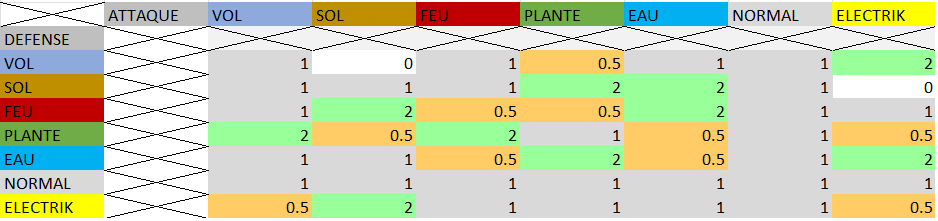
\includegraphics[width=15cm,height=4cm]{images/tableau_type}
		\end{center}
        Voici un tableau presentant les rapports entre les différents types:
        \begin{itemize}
        \item Se lit " le type 1 (colonne) est en faiblesse, resistance, immunité ou normal par rapport au type 2 (ligne) si le coefficient est respectivement 2, 0.5, 0 ou 1
        \end{itemize}